\documentclass{article}
\usepackage{color}
\usepackage{tikz}
\usepackage{float}
\usepackage{tabularx}
\usepackage{amsmath}
\usepackage{amssymb}
\usepackage{listings}
\usepackage{enumitem}
\usepackage{syntax}
\usepackage{csquotes}
\usepackage[backend=biber]{biblatex}
\addbibresource{references.bib}

\usepackage{tikz}
\usetikzlibrary{automata,positioning}
\tikzset{
  gray box/.style={
    fill=gray!20,
    draw=gray,
    minimum width={2*#1ex},
    minimum height={2em},
  },
  annotation/.style={
    anchor=north,
  }
}


\definecolor{dkgreen}{rgb}{0,0.6,0}
\definecolor{gray}{rgb}{0.5,0.5,0.5}
\definecolor{mauve}{rgb}{0.58,0,0.82}


\lstset{frame=tb,
  numbers=left,
  stepnumber=1,
  language=Java,
  aboveskip=3mm,
  belowskip=3mm,
  showstringspaces=false,
  columns=flexible,
  basicstyle={\small\ttfamily},
  numberstyle=\color{gray},
  keywordstyle=\color{blue},
  commentstyle=\color{dkgreen},
  stringstyle=\color{mauve},
  breaklines=true,
  breakatwhitespace=true,
  tabsize=2,
  moredelim=**[is][\color{red}]{@}{@},
}

\setlength{\grammarindent}{12em}

%\renewcommand{\lstlistingname}{Algorithm}
%\newcommand{\tablerow}[4]{ #1 & #2 & #3 & #4\\}
\newcommand{\n}[0]{\\[\baselineskip]}
%\newcommand{\qa}[2]{\textbf{Q:} #1 \\ \textbf{A:} #2}
%\newcommand{\argument}[4]{\textbf{#1:} #2 \\ \textbf{#3:} #4}

\title{CS4202 Computer Architecture - Process Scheduling for Heterogeneous Systems}
\author{140011146}

\begin{document}

\maketitle

\section{Introduction}
CPU scheduling is vital for the multitasking environment of modern operating systems. Processes waiting for I/O can be switched out to prevent wasted CPU cycles, but any process can be pre-empted for better user interactivity, efficiency and fairness \cite{os}. As a result, it is important to understand the effects of scheduling on performance.
\n
First, a round-robin scheduling approach for CPUs is looked into, discussing how the approach works and where the approach performs well or poorly. 
\n
Next, a genetic algorithm was implemented to explore the search space of possible schedules with the GEM5 simulator on two benchmarks. The schedules produced by the genetic algorithm are then compared with both the default approach of the simulator and from a completely random schedule to gain an understanding of the scheduling optimisation space.

\section{Task 1 - Round-robin scheduling}
The round-robin CPU scheduling approach is similar to a simple First-Come First-Served scheduling approach, but all processes bursts are limited by a time quantum. Processes will be pre-empted if they run longer than the time quantum to give the next processes in the queue a chance to run. Processes that make an I/O request or finish before the time quantum are also moved off the CPU \cite{rr-paper}.
\n
A circular queue of processes that are ready to be executed is maintained by the scheduler. New processes join at the end of the queue. The scheduler chooses and removes the first process in the queue and after the processes has finished its time quantum it is moved back to the end of the queue. For example, consider the following processes in the ready queue.
\n
\begin{figure}[H]
\centering
\begin{tabular}{c c}
\textbf{Process} & \textbf{Burst time} \\
\hline
$P_{1}$ & 17 \\
$P_{2}$ & 3 \\
$P_{3}$ & 4 \\
\end{tabular}
\end{figure}
\noindent 
A time quantum of 3 would result in the following schedule and wait times:
\begin{figure}[H]
\centering
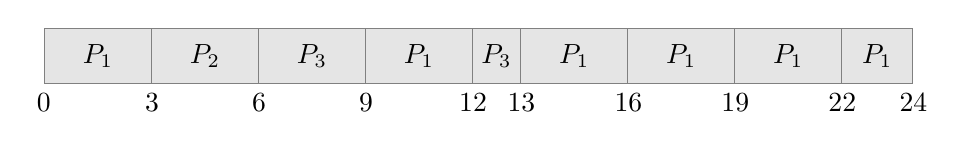
\begin{tikzpicture}[node distance=-0.5pt]
  \node [gray box=4.5] (p1) {\(P_{1}\)};
  \node [gray box=4.5, right=of p1] (p2) {\(P_{2}\)};
  \node [gray box=4.5, right=of p2] (p3) {\(P_{3}\)};
  \node [gray box=4.5, right=of p3] (p4) {\(P_{1}\)};
  \node [gray box=1.5, right=of p4] (p5) {\(P_{3}\)};
  \node [gray box=4.5, right=of p5] (p6) {\(P_{1}\)};
  \node [gray box=4.5, right=of p6] (p7) {\(P_{1}\)};
  \node [gray box=4.5, right=of p7] (p8) {\(P_{1}\)};
  \node [gray box=3, right=of p8] (p9) {\(P_{1}\)};

  \node [annotation] at (p1.south west) {0};
  \node [annotation] at (p1.south east) {3};
  \node [annotation] at (p2.south east) {6};
  \node [annotation] at (p3.south east) {9};
  \node [annotation] at (p4.south east) {12};
  \node [annotation] at (p5.south east) {13};
  \node [annotation] at (p6.south east) {16};
  \node [annotation] at (p7.south east) {19};
  \node [annotation] at (p8.south east) {22};
  \node [annotation] at (p9.south east) {24};
\end{tikzpicture}
\caption{Schedule with a time quantum of 3}
\end{figure}
\noindent Wait times:
\begin{itemize}
\item $P_{1}$: 7 time units
\item $P_{2}$: 3 time units
\item $P_{3}$: 9 time units
\end{itemize}
\noindent Average wait time = $19 / 3 = 6.33$ time units.
\n
However, a time quantum of 10 would result in a much longer average wait time.
\begin{figure}[H]
\centering
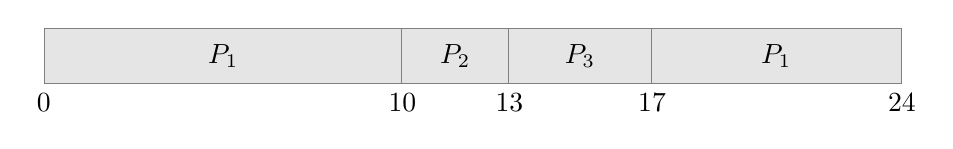
\begin{tikzpicture}[node distance=-0.5pt]
  \node [gray box=15] (p1) {\(P_{1}\)};
  \node [gray box=4.5, right=of p1] (p2) {\(P_{2}\)};
  \node [gray box=6, right=of p2] (p3) {\(P_{3}\)};
  \node [gray box=10.5, right=of p3] (p4) {\(P_{1}\)};

  \node [annotation] at (p1.south west) {0};
  \node [annotation] at (p1.south east) {10};
  \node [annotation] at (p2.south east) {13};
  \node [annotation] at (p3.south east) {17};
  \node [annotation] at (p4.south east) {24};
\end{tikzpicture}
\caption{Schedule with a time quantum of 10}
\end{figure}
\noindent Wait times:
\begin{itemize}
\item $P_{1}$: 7 time units
\item $P_{2}$: 10 time units
\item $P_{3}$: 13 time units
\end{itemize}
\noindent Average wait time = $30 / 3 = 10$ time units.
\n
Changing the size of the time quantum affected the average waiting time, as process 2 and 3 had to wait much longer before getting a chance to run. However, this comes at a trade-off of less context switches. With a quantum of 10, only 3 context switches were required, whereas with a quantum of 3, 8 context switches were required. Context switches can be expensive as they take up computation and time, especially for switching between processes. Although the exact cost of context switches depends on the processor and operating system
\n
An issue with the simple round-robin scheduling approach is the long average waiting time. Given $n$ processes in the ready queue with a time quantum of $t$, each process only gets $t$ time to run every $nt$ time units and must wait at most $(n - 1) \times t$ before each turn. Therefore, the length of the time quantum heavily impacts the performance of the round-robin approach. A very long time quantum will effectively be the same as a FCFS approach, resulting in poor response and waiting time if there are processes with long bursts. On the other hand, a very short time quantum results in a large overhead of many context switches between the processes, wasting time and CPU cycles on context switching rather than useful computation. 
\n
Round-robin performs well for load balancing if the processes all have similar bursts times. 
\n
Some processes want/should have more share of the processor than others (concept for priority)
\n
Long queue leads to high response time and high turnaround time as a simple round-robin approach adds new processes to the tail of the queue, giving a response time of at most $(n - 1) \times t$ time units where $n$ is the number of processes in the queue and $t$ is the time quantum.
\section{Task 2}

\subsection{Methodology}
A genetic algorithm was chosen as a means to explore the search space of binary schedules. Because of the large optimisation space of schedules, a genetic algorithm with mutation adds elements of randomness to help explore more of the search space compared to a hill climbing algorithm which can get easily stuck in local maxima. Furthermore, hill climbing with random restart will only try to explore another unrelated area of the search space for a maximum without taking into account the previous local maxima. 
\n
The binary schedules are deterministic, that is to say the same schedule will always take the same time to run. Additionally, if two schedules share the same initial $n$ bits, they will run identically until they differ. This means that where the bits change in the binary stream matters. Given a binary schedule, if the first few bits are modified, the schedule will be completely different. If only the last few bits are modified, then the schedule is only different at those last few bits.
\n
instead of some form of hill-climbing algorithm
- no obvious direction for climbing  higher, unclear how to change bits except going through all, which would be too many combinations
- easy to fall into local minimum 
- eg if only change lower half of schedule, not exploring changing the top half
- randomly restart top half to escape minima doesn't work because affects entire schedule
- ga with crossover reproduction allows exploring different "better" top halves of the schedule
- mutation avoids local minima

- issue with ga is a bit slow to converge and may miss some maxima

- because we don't know how schedule affects time, unsure if crossover/selection/mutation strategies are suitable

Improvements on GA:
- increased population
- crossover only top halves of parents
- increased mutation due to local minima
- increased/decreased tournament selection size
- less or no elites

Increased population due to stagnation at local maxima for more diversity and less likely to choose similar parents in population

Larger population explores more of the search space, but converges slower

Increased mutation also due to local maxima. Perhaps crossover is not effective because if the schedule is good, only some portion of the top half of the binary is used, so low mutation rate where mutation happens in lower half has no effect.

-> Change crossover to must be halfway point or above? -> Prevent low crossover point which has little effect

Elites introduced to keep good schedules, number of elites randomised so not always the same 

Smaller tournament size to allow weak individuals to increase more diversity
Larger tournament size means more likely to have strong individuals for faster convergence

Optimise size of schedule as much as possible to prevent entire lower half being unused


- if schedule is too short, then the simulator will fail and return 0 for that fitness -> this allows removing potential bad schedules

\subsection{Experimentation}
\subsubsection{Experiment 1}
In the first na\"{i}ve experiment, the following parameters were chosen:
\begin{itemize}
\item \textbf{Population size}: 25
\item \textbf{Chromosome length}: 100000
\item \textbf{Mutation probability per gene}: $\dfrac{1}{(l/10)}$ where $l$ is the length of the chromosome
\item \textbf{Crossover point}: Random
\item \textbf{Selection}: Tournament with 3 competitors
\end{itemize}
The population size was chosen as a size that was not too small or too large to start with. Fine tuning the population size for the specific task of finding a fast schedule will require more work, but starting with a medium sized population will give an indication as to whether this is too small or too large. A population that is too small will be stuck in a local maximum and unable to find better solutions, while a population that is too large would lead to a slow rate of convergence \cite{ga-size}. 
\subsubsection{Experiment 2}

\subsection{Results}

\subsection{Evaluation}

\printbibliography

\end{document}



